% =====================================================================
% RTC 2027 Student 3K -- Raspberry Pi Pico electronics MDR contribution
% Build:  pdflatex -> biber -> pdflatex -> pdflatex   (Overleaf does this automatically)
% The BibTeX database is embedded below (filecontents*) and is written to
% RTC_2027_Pico_MDR_refs.bib on the first run, so it will not overwrite
% your existing RTC_2027_Electronics_MDR_Draft.bib.
% =====================================================================

\begin{filecontents*}[overwrite]{RTC_2027_Pico_MDR_refs.bib}
% ---------------- Organiser documents (uploaded RTC package) ----------------
@misc{rtc2027app01,
  author = {{RTC 2027 Organiser}},
  title  = {Appendix 01: Mission Plan Report example and slide template},
  year   = {2026},
  note   = {Competition document, \texttt{appendix\_01.pptx}}
}
@misc{rtc2027app03,
  author = {{RTC 2027 Organiser}},
  title  = {Appendix 03: Rocket Design Specifications},
  year   = {2026},
  note   = {Competition document, \texttt{appendix\_03.pdf}}
}
@misc{rtc2027app06,
  author = {{RTC 2027 Organiser}},
  title  = {Appendix 06: Competition Rules Explanation, version 2},
  year   = {2026},
  note   = {Competition document, \texttt{appendix\_06.pdf}}
}
@misc{rtc2027app07,
  author = {{RTC 2027 Organiser}},
  title  = {Appendix 07: MDR scoring and Design Maturity Matrix},
  year   = {2026},
  note   = {Competition document, \texttt{appendix\_07.xlsx}}
}
@misc{rtc2027app08,
  author = {{RTC 2027 Organiser}},
  title  = {Appendix 08: Launch Permit Inspection Checklist},
  year   = {2026},
  note   = {Competition document, \texttt{appendix\_08.xlsx}}
}
@misc{rtc2027app12,
  author = {{RTC 2027 Organiser}},
  title  = {Appendix 12: FMEA Example},
  year   = {2026},
  note   = {Competition document, \texttt{appendix\_12.xlsx}}
}
% ---------------- Manufacturer documentation ----------------
@manual{rp2040ds,
  author       = {{Raspberry Pi Ltd}},
  title        = {{RP2040} Datasheet: A Microcontroller by {Raspberry Pi}},
  year         = {2024},
  url          = {https://datasheets.raspberrypi.com/rp2040/rp2040-datasheet.pdf},
  urldate      = {2026-11-04}
}
@manual{picods,
  author       = {{Raspberry Pi Ltd}},
  title        = {Raspberry {Pi} {Pico} Datasheet: An {RP2040}-based Microcontroller Board},
  year         = {2024},
  url          = {https://datasheets.raspberrypi.com/pico/pico-datasheet.pdf},
  urldate      = {2026-11-04}
}
@manual{rp2040hw,
  author       = {{Raspberry Pi Ltd}},
  title        = {Hardware Design with {RP2040}},
  year         = {2024},
  url          = {https://datasheets.raspberrypi.com/rp2040/hardware-design-with-rp2040.pdf},
  urldate      = {2026-11-04}
}
@manual{picosdk,
  author       = {{Raspberry Pi Ltd}},
  title        = {Raspberry {Pi} {Pico}-series {C/C++} {SDK}},
  year         = {2024},
  url          = {https://datasheets.raspberrypi.com/pico/raspberry-pi-pico-c-sdk.pdf},
  urldate      = {2026-11-04}
}
@manual{bmp280ds,
  author       = {{Bosch Sensortec GmbH}},
  title        = {{BMP280} Digital Pressure Sensor Datasheet},
  number       = {BST-BMP280-DS001},
  year         = {2018},
  url          = {https://www.bosch-sensortec.com/products/environmental-sensors/pressure-sensors/bmp280/},
  urldate      = {2026-11-04}
}
@manual{mpu6050ds,
  author       = {{InvenSense Inc.}},
  title        = {{MPU-6000} and {MPU-6050} Product Specification, Revision 3.4},
  number       = {PS-MPU-6000A-00},
  year         = {2013},
  url          = {https://invensense.tdk.com/products/motion-tracking/6-axis/mpu-6050/},
  urldate      = {2026-11-04}
}
@manual{ds18b20ds,
  author       = {{Maxim Integrated}},
  title        = {{DS18B20} Programmable Resolution 1-Wire Digital Thermometer},
  year         = {2019},
  url          = {https://www.analog.com/media/en/technical-documentation/data-sheets/ds18b20.pdf},
  urldate      = {2026-11-04}
}
@manual{adxl375ds,
  author       = {{Analog Devices}},
  title        = {{ADXL375}: 3-Axis, $\pm$200 g Digital {MEMS} Accelerometer},
  year         = {2020},
  url          = {https://www.analog.com/en/products/adxl375.html},
  urldate      = {2026-11-04}
}
@manual{atmega328ds,
  author       = {{Microchip Technology}},
  title        = {{ATmega328P} Data Sheet},
  number       = {DS40002061},
  year         = {2020},
  url          = {https://www.microchip.com/en-us/product/ATmega328P},
  urldate      = {2026-11-04}
}
@manual{esp32ds,
  author       = {{Espressif Systems}},
  title        = {{ESP32} Series Datasheet},
  year         = {2024},
  url          = {https://www.espressif.com/en/support/documents/technical-documents},
  urldate      = {2026-11-04}
}
@manual{i2cspec,
  author       = {{NXP Semiconductors}},
  title        = {{I2C}-bus Specification and User Manual, Rev. 7.0},
  number       = {UM10204},
  year         = {2021},
  url          = {https://www.nxp.com/docs/en/user-guide/UM10204.pdf},
  urldate      = {2026-11-04}
}
@manual{sdspec,
  author       = {{SD Association}},
  title        = {{SD} Specifications Part 1: Physical Layer Simplified Specification},
  year         = {2020},
  note         = {Use the current published version; SPI-mode command set is defined in this document},
  url          = {https://www.sdcard.org/downloads/pls/},
  urldate      = {2026-11-04}
}
@misc{fatfs,
  author       = {Chan, Hiroaki},
  title        = {{FatFs} -- Generic {FAT} Filesystem Module},
  howpublished = {Online documentation},
  url          = {http://elm-chan.org/fsw/ff/},
  urldate      = {2026-11-04}
}
% ---------------- Systems engineering / reliability ----------------
@manual{nasase,
  author       = {{NASA}},
  title        = {{NASA} Systems Engineering Handbook},
  number       = {NASA/SP-2016-6105 Rev2},
  year         = {2016},
  url          = {https://www.nasa.gov/reference/systems-engineering-handbook/},
  urldate      = {2026-11-04}
}
@manual{mil1629a,
  author       = {{US Department of Defense}},
  title        = {Procedures for Performing a Failure Mode, Effects and Criticality Analysis},
  number       = {MIL-STD-1629A},
  year         = {1980}
}
\end{filecontents*}

\documentclass[10pt,a4paper]{article}
\usepackage[a4paper,margin=17mm,top=18mm,bottom=18mm]{geometry}
\usepackage[T1]{fontenc}
\usepackage[utf8]{inputenc}
\usepackage{lmodern,microtype}
\usepackage[table]{xcolor}
\usepackage{booktabs,tabularx,longtable,array}
\usepackage{enumitem}
\usepackage{tikz}
\usetikzlibrary{arrows.meta,positioning,shapes.geometric,calc}
\usepackage{csquotes}
\usepackage[unicode,colorlinks=true,linkcolor=blue!55!black,urlcolor=blue!55!black,citecolor=blue!55!black]{hyperref}
\usepackage[backend=biber,style=ieee,sorting=none,maxnames=5]{biblatex}
\addbibresource{RTC_2027_Pico_MDR_refs.bib}
\usepackage{fancyhdr,titlesec}
\usepackage{ragged2e}
\usepackage{caption}
\captionsetup{font=small,labelfont=bf}

\definecolor{Navy}{HTML}{12304A}
\definecolor{Teal}{HTML}{067A80}
\definecolor{Pale}{HTML}{EFF5F8}
\definecolor{VeryLight}{HTML}{E8F1F6}
\definecolor{Amber}{HTML}{8A5714}
\hypersetup{pdftitle={RTC 2027 Student 3K - Electronics MDR Contribution}}

\titleformat{\section}{\large\bfseries\color{Navy}}{\thesection.}{.6em}{}
\titleformat{\subsection}{\normalsize\bfseries\color{Teal}}{\thesubsection}{.6em}{}
\titlespacing*{\section}{0pt}{12pt}{5pt}
\titlespacing*{\subsection}{0pt}{8pt}{4pt}
\setlength{\parindent}{0pt}
\setlength{\parskip}{4pt}
\setlength{\emergencystretch}{2em}
\setlist[itemize]{topsep=2pt,itemsep=1pt,leftmargin=1.2em}
\setlist[enumerate]{topsep=2pt,itemsep=1pt,leftmargin=1.3em}
\newcolumntype{L}[1]{>{\RaggedRight\arraybackslash}p{#1}}
\newcolumntype{Y}{>{\RaggedRight\arraybackslash}X}
\newcommand{\status}[1]{{\footnotesize\textcolor{Amber}{#1}}}

\pagestyle{fancy}\fancyhf{}
\fancyhead[L]{\footnotesize\color{Teal}RTC 2027 | Student 3K | Electronics}
\fancyhead[R]{\footnotesize\color{gray}Pico-based MDR contribution | 4 Nov 2026}
\fancyfoot[C]{\footnotesize\thepage}
\renewcommand{\headrulewidth}{.3pt}

% ---------- TikZ flowchart styles ----------
\tikzset{
  >=Latex,
  term/.style={draw=Navy,rounded corners=7pt,fill=Navy!10,align=center,font=\scriptsize\bfseries,text width=4.2cm,minimum height=7mm,inner sep=2pt},
  proc/.style={draw=Navy!70,rounded corners=1.5pt,fill=Pale,align=center,font=\scriptsize,text width=5cm,minimum height=8mm,inner sep=2.5pt},
  dec/.style={draw=Teal,diamond,aspect=2.4,fill=Teal!8,align=center,font=\scriptsize,text width=2.2cm,inner sep=1pt},
  fault/.style={draw=Amber,rounded corners=1.5pt,fill=Amber!10,align=center,font=\scriptsize,text width=3.4cm,minimum height=8mm,inner sep=2.5pt},
  note/.style={draw=gray,dashed,rounded corners=1.5pt,fill=white,align=left,font=\scriptsize,text width=3.4cm,inner sep=2.5pt},
  conn/.style={draw=Navy,circle,fill=Navy!10,font=\scriptsize\bfseries,inner sep=1.5pt},
  flow/.style={-Latex,semithick,color=Navy!75},
  lab/.style={font=\tiny\bfseries,color=Teal,inner sep=1.5pt},
  group/.style={draw=Teal,dashed,rounded corners=3pt},
  lane/.style={draw=Navy!30,fill=Pale!55,rounded corners=2pt}
}

\begin{document}

\begin{center}
{\small\bfseries\color{Teal}PRELIMINARY DESIGN -- FOR MDR INTEGRATION}\par\vspace{3pt}
{\LARGE\bfseries\color{Navy}Raspberry Pi Pico Electronics Architecture}\par\vspace{2pt}
{\large Process flow, component rationale and 3K design-criteria fit}\par\vspace{4pt}
{\small RTC 2027 Student 3K | Mission Design Report: electronics contribution | 4 November 2026}\par
\end{center}
\vspace{-1mm}\hrule\vspace{3mm}

\fcolorbox{Teal!35}{Pale}{\parbox{.955\linewidth}{\small\textbf{Scope and status.} This is the electronics team's contribution draft to the team's single MDR; it is not a separately submitted report and not a completed flight design. Competition constraints are attributed to the organiser documents \cite{rtc2027app03,rtc2027app06,rtc2027app07}. Thresholds, rates, pin allocations, power figures and the thermal payload are \emph{team proposals} marked as such, and require simulation, approval and later testing in line with the MDR/PDR/CDR maturity expectations \cite{rtc2027app07,nasase}. Manufacturer figures are quoted from the cited datasheets and should be re-checked against the exact module purchased.}}

%======================================================================
\section{Design drivers: how the Pico design meets the 3K criteria}
%======================================================================
The design uses \textbf{three separate Raspberry Pi Pico boards} (RP2040) \cite{picods,rp2040ds}: one \emph{logger/payload} Pico that never commands recovery, and two \emph{independent recovery} Picos (primary and backup), each with its own barometer and battery. This keeps required flight-data logging and the thermal experiment from sharing a failure path with parachute deployment, while using one familiar, low-cost, well-documented platform for every computer in the rocket.

\small
\rowcolors{2}{Pale}{white}
\begin{longtable}{@{}L{34mm}L{70mm}L{46mm}@{}}
\toprule\rowcolor{VeryLight}\textbf{3K criterion}&\textbf{Design response}&\textbf{Basis / status}\\\midrule\endfirsthead
\toprule\rowcolor{VeryLight}\textbf{3K criterion}&\textbf{Design response (continued)}&\textbf{Basis / status}\\\midrule\endhead
\bottomrule\endlastfoot
Record altitude, velocity, acceleration, GPS trajectory & Logger Pico records BMP280 pressure-altitude and MPU6050 acceleration with timestamps; velocity is derived by filtering/fusion; GPS track is taken from the organiser beacon as a separate dataset. & \cite{rtc2027app03} Sec.~2.1; proposed method\\
Detect launch, apogee, descent & Multi-condition state machine (Figs.~\ref{fig:boot}--\ref{fig:flight}) with lock-outs and time-out back-ups. & \cite{rtc2027app03} Sec.~4.2.2.4; proposed\\
Two-stage recovery: drogue at apogee, main at lower altitude & Two recovery Picos each execute both events; main altitude selected in the 150--450\,m window, below the 500\,m inspection criterion. & \cite{rtc2027app03} 4.2.2.4; \cite{rtc2027app08} Row 8\\
Independent / redundant activation, release redundancy & Primary and backup recovery Picos, separate batteries, separate barometers, outputs held low in hardware (Fig.~\ref{fig:recovery}). & \cite{rtc2027app03} 4.1.3, 4.2.2.2; mechanism \status{TBD}\\
Safe/armed states, arming confirmation & Arming switch gates power; outputs forced low by pull-downs; launch-inhibit logic; buzzer/LED status code. & \cite{rtc2027app03} 4.6.3--4.6.7\\
Vibration, impact, sensor error & Plausibility gates, filtering, CRC records, strain-relieved connectors, watchdog warm restart. & \cite{rtc2027app03} 4.1.2, 4.4\\
$>1.5$\,h electrical operation & Single Li-ion cell per Pico; load $\approx$56\,mA estimated, 200\,mA design basis (Sec.~\ref{sec:power}). & \cite{rtc2027app03} 4.7.2; \cite{rtc2027app08} Row 6\\
Official GPS tracker & Separate, organiser-standard beacon, own power, no electrical dependence on Pico boards. & \cite{rtc2027app03} 2.2, 5.1\\
Additional payload & Two DS18B20 probes read by the logger Pico: internal avionics-bay vs inner-wall temperature difference; retained in rocket, no radio, no stored-energy device. & \cite{rtc2027app03} 7.1; team proposal\\
No unapproved radio emissions & Plain Pico (not Pico~W): no on-board radio. & \cite{rtc2027app03} 4.1.4; \cite{picods}\\
\end{longtable}
\normalsize

%======================================================================
\section{System architecture}
%======================================================================
\begin{figure}[ht]
\centering
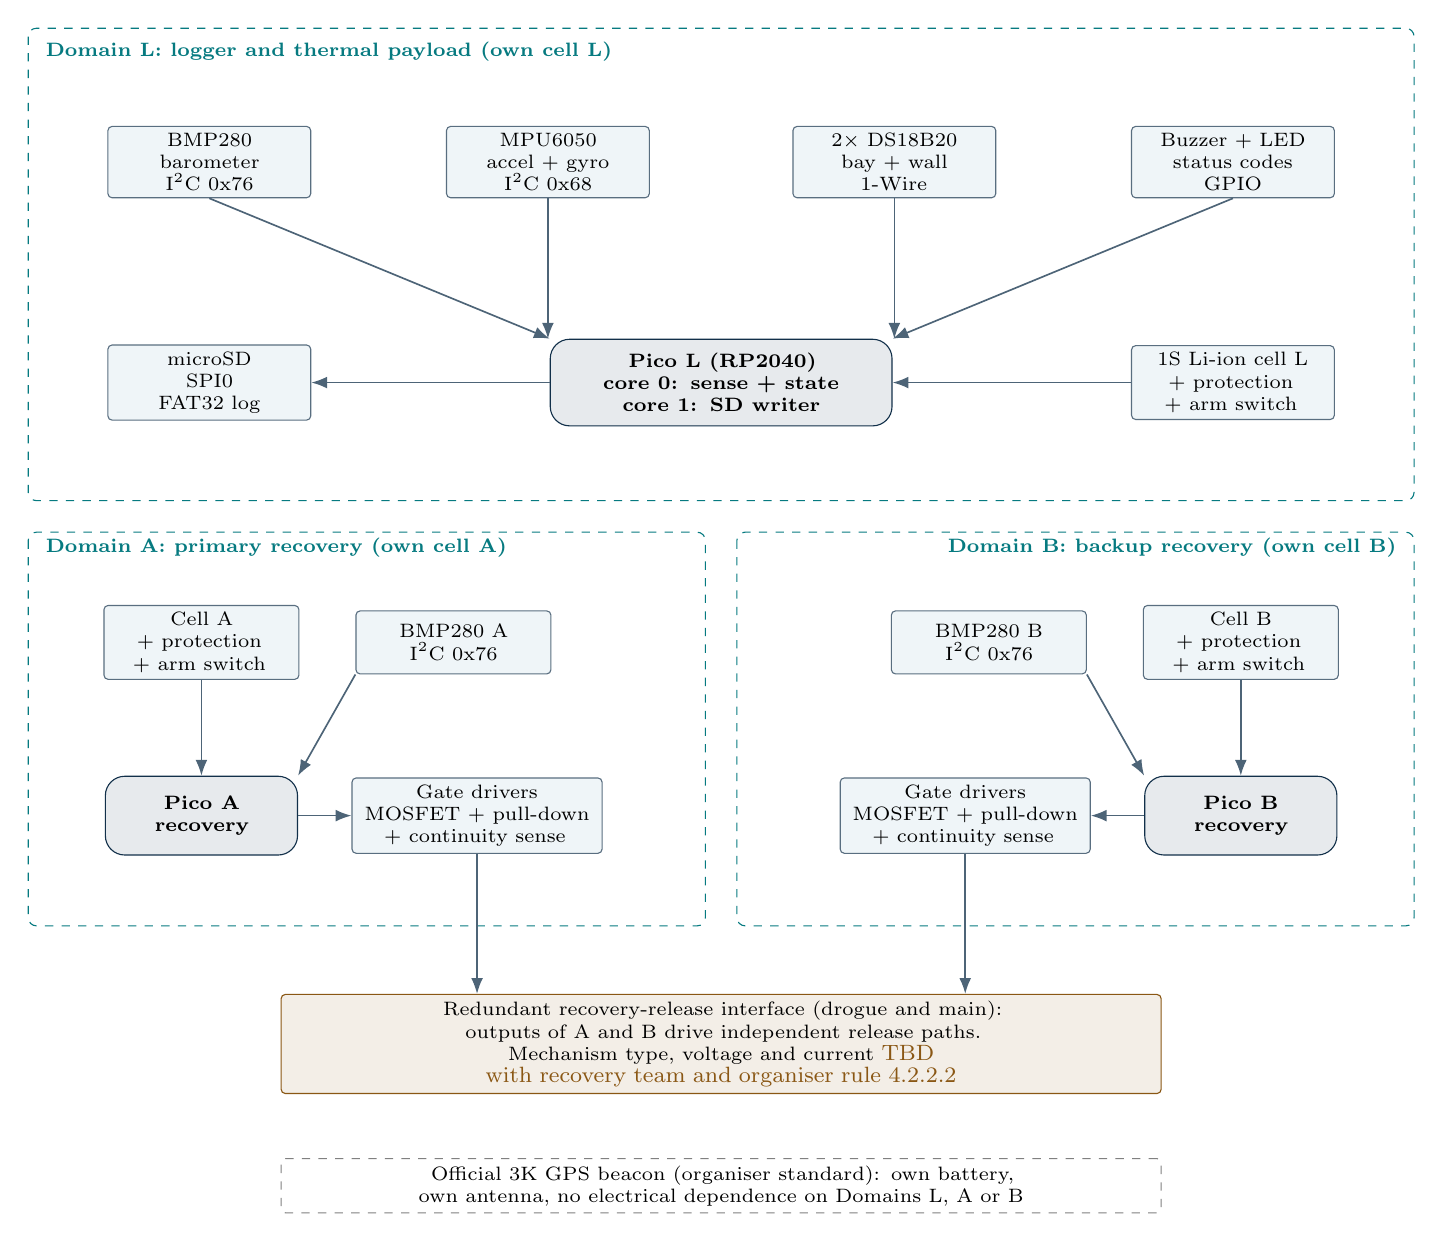
\begin{tikzpicture}[font=\scriptsize]
% ---- logger domain ----
\draw[group] (-8.8,1.0) rectangle (8.8,-5.0);
\node[font=\scriptsize\bfseries,color=Teal,anchor=north west] at (-8.7,0.95) {Domain L: logger and thermal payload (own cell L)};
\node[proc,text width=2.4cm] (bmpL) at (-6.5,-0.7) {BMP280\\barometer\\I$^2$C 0x76};
\node[proc,text width=2.4cm] (mpu)  at (-2.2,-0.7) {MPU6050\\accel + gyro\\I$^2$C 0x68};
\node[proc,text width=2.4cm] (ds)   at (2.2,-0.7)  {2$\times$ DS18B20\\bay + wall\\1-Wire};
\node[proc,text width=2.4cm] (bz)   at (6.5,-0.7)  {Buzzer + LED\\status codes\\GPIO};
\node[term,text width=4.2cm,minimum height=11mm] (picoL) at (0,-3.5) {Pico L (RP2040)\\core 0: sense + state\\core 1: SD writer};
\node[proc,text width=2.4cm] (sd)   at (-6.5,-3.5) {microSD\\SPI0\\FAT32 log};
\node[proc,text width=2.4cm] (batL) at (6.5,-3.5)  {1S Li-ion cell L\\+ protection\\+ arm switch};
\draw[flow] (bmpL.south) -- (picoL.north west);
\draw[flow] (mpu.south) -- (mpu.south |- picoL.north);
\draw[flow] (ds.south) -- (ds.south |- picoL.north);
\draw[flow] (bz.south) -- (picoL.north east);
\draw[flow] (picoL.west) -- (sd.east);
\draw[flow] (batL.west) -- (picoL.east);
% ---- recovery domains ----
\foreach \s/\n/\x/\ba/\bb/\pa/\pb in {-1/A/-6.6/south west/north east/east/west, 1/B/6.6/south east/north west/west/east} {
  \node[proc,text width=2.3cm] (bat\n) at (\x,-6.8) {Cell \n\\+ protection\\+ arm switch};
  \node[proc,text width=2.3cm] (bmp\n) at (\s*3.4,-6.8) {BMP280 \n\\I$^2$C 0x76};
  \node[term,text width=2.3cm,minimum height=10mm] (pico\n) at (\x,-9.0) {Pico \n\\recovery};
  \node[proc,text width=3.0cm] (drv\n) at (\s*3.1,-9.0) {Gate drivers\\MOSFET + pull-down\\+ continuity sense};
  \draw[flow] (bat\n.south) -- (pico\n.north);
  \draw[flow] (bmp\n.\ba) -- (pico\n.\bb);
  \draw[flow] (pico\n.\pa) -- (drv\n.\pb);
}
\draw[group] (-8.8,-5.4) rectangle (-0.2,-10.4);
\draw[group] (0.2,-5.4) rectangle (8.8,-10.4);
\node[font=\scriptsize\bfseries,color=Teal,anchor=north west] at (-8.7,-5.35) {Domain A: primary recovery (own cell A)};
\node[font=\scriptsize\bfseries,color=Teal,anchor=north east] at (8.7,-5.35) {Domain B: backup recovery (own cell B)};
\node[fault,text width=11cm] (rel) at (0,-11.9) {Redundant recovery-release interface (drogue and main): outputs of A and B drive independent release paths.\\Mechanism type, voltage and current \status{TBD with recovery team and organiser rule 4.2.2.2}};
\draw[flow] (drvA.south) -- (drvA.south |- rel.north);
\draw[flow] (drvB.south) -- (drvB.south |- rel.north);
\node[note,text width=11cm,align=center] (gps) at (0,-13.7) {Official 3K GPS beacon (organiser standard): own battery, own antenna, no electrical dependence on Domains L, A or B};
\end{tikzpicture}
\caption{Electronics architecture. Three Pico boards in three power domains; the logger can fail without affecting recovery, and recovery A can fail without affecting recovery B. Illustrative; wiring and fault independence remain to be approved.}
\label{fig:arch}
\end{figure}

\textbf{Critical interface rule.} The logger never commands recovery, and nothing on Domain~L (SD card, thermal probes, buzzer) can block a recovery decision. Cross-links between domains are limited to a common ground reference at the release interface if the recovery team requires it; no shared supply \cite{rtc2027app03}.

%======================================================================
\section{Why the Raspberry Pi Pico}
%======================================================================
\small
\rowcolors{2}{Pale}{white}
\begin{longtable}{@{}L{36mm}L{58mm}L{56mm}@{}}
\toprule\rowcolor{VeryLight}\textbf{RP2040 / Pico feature}&\textbf{What it provides}&\textbf{Benefit to the 3K rocket}\\\midrule\endfirsthead
\toprule\rowcolor{VeryLight}\textbf{Feature}&\textbf{What it provides}&\textbf{Benefit (continued)}\\\midrule\endhead
\bottomrule\endlastfoot
Dual Cortex-M0+ cores, up to 133\,MHz & Two independent cores sharing memory \cite{rp2040ds}. & Core~0 senses and decides; core~1 does slow SD writes, so storage latency cannot delay sampling (Fig.~\ref{fig:loop}).\\
264\,kB on-chip SRAM & Fast RAM for buffers \cite{rp2040ds}. & A 5\,s pre-trigger and write-ahead buffer at 24\,B $\times$ 200\,Hz uses about 24\,kB ($\approx$9\% of SRAM).\\
Hardware I$^2$C, SPI, UART, ADC & Two I$^2$C, two SPI, two UART, 12-bit ADC inputs \cite{rp2040ds}. & Covers IMU/baro (I$^2$C), SD (SPI) and battery-voltage monitoring without extra chips.\\
Programmable I/O (PIO) & Eight state machines for custom protocols \cite{rp2040ds}. & Cycle-exact 1-Wire for DS18B20 without blocking the CPU.\\
Watchdog with scratch registers & Reset timer; scratch registers survive a watchdog reset \cite{rp2040ds}. & In-flight reset recovers flight state (Fig.~\ref{fig:boot}): robustness against vibration/brown-out glitches.\\
Wide supply: VSYS 1.8--5.5\,V & On-board buck-boost supply to 3.3\,V \cite{picods}. & A single 3.0--4.2\,V Li-ion cell powers the board directly; the rail holds as the cell discharges.\\
No radio (Pico, not Pico~W) & Plain board without Wi-Fi/Bluetooth \cite{picods}. & Avoids unapproved emissions from the rocket \cite{rtc2027app03}.\\
Open C/C++ SDK, SWD debug, UF2 boot & Free toolchain and bootloader \cite{picosdk}. & Rapid iteration, scripted builds, and the same toolchain on all three boards.\\
Low cost and availability & Retail boards at a few ringgit, drop-in spares. & Three flight computers plus spares fit a student budget; identical hardware simplifies sparing.\\
\end{longtable}
\normalsize

\textbf{Alternatives considered.} An 8-bit AVR such as the ATmega328P has only 2\,kB of SRAM \cite{atmega328ds}, too little for a buffered logger plus filtering. ESP32 devices offer more processing but include Wi-Fi/Bluetooth radios \cite{esp32ds} that must be disabled or justified under the radio rules \cite{rtc2027app03}. The Pico gives enough memory and I/O without a radio at similar cost.

\textbf{Known Pico limits and mitigations.} The Cortex-M0+ has no hardware FPU \cite{rp2040ds}; at 200\,Hz the filter workload is small, but fixed-point or measured float timing will be checked. Flash is external (XIP), so \emph{no flash writes during flight}; recovery events are kept in RAM and dumped after landing \cite{rp2040ds,picosdk}. A Pico dev board is not qualified flight hardware: the independence of A and B, the watchdog, hard-wired pull-downs and testing are what give confidence, not the board itself. The Pico operating range is $-20$ to $+85\,^{\circ}$C \cite{picods}; the bay temperature is measured by the payload.

%======================================================================
\section{Component-by-component rationale}
%======================================================================
\small
\rowcolors{2}{Pale}{white}
\begin{longtable}{@{}L{23mm}L{30mm}L{60mm}L{37mm}@{}}
\toprule\rowcolor{VeryLight}\textbf{Component}&\textbf{Role}&\textbf{Rationale and fit to 3K criteria}&\textbf{Limit / mitigation}\\\midrule\endfirsthead
\toprule\rowcolor{VeryLight}\textbf{Component}&\textbf{Role}&\textbf{Rationale (continued)}&\textbf{Limit / mitigation}\\\midrule\endhead
\bottomrule\endlastfoot
Pico L (logger) & Flight data, state estimate, thermal payload, status. & Satisfies mandatory output list \cite{rtc2027app03}; isolates non-safety functions from recovery. & Not a recovery path. Verified by Fig.~\ref{fig:arch} separation.\\
Pico A / Pico B (recovery) & Independent apogee and main-altitude logic and output control. & Redundant activation and release redundancy \cite{rtc2027app03}; identical code base reduces effort, separate boards and cells remove single points of failure. & Common-mode software bug: backup uses different thresholds and delay (Sec.~\ref{tab:params}).\\
BMP280 (one per Pico) & Pressure/temperature $\rightarrow$ altitude. & Pressure range 300--1100\,hPa covers sea level to well above 3\,km ($\approx$701\,hPa at 3\,km in a standard atmosphere); relative accuracy about $\pm0.12$\,hPa ($\approx\pm1$\,m) \cite{bmp280ds}. Barometric altitude is the standard method for apogee and main-deployment decisions. & Port must see static pressure, vented away from fast airflow; lock-out near burnout/transonic transients; absolute offset removed by pad baseline.\\
MPU6050 & Acceleration (and angular rate) for launch/burnout detection and acceleration record. & 16-bit ADC, programmable $\pm2$ to $\pm16$\,g, 400\,kHz I$^2$C \cite{mpu6050ds,i2cspec}; $\pm16$\,g gives 2048\,LSB/g, ample resolution. & May saturate during boost: optional $\pm200$\,g ADXL375 \cite{adxl375ds} if simulation shows $>16$\,g; gyro $\pm2000^{\circ}$/s limits roll-rate capture.\\
DS18B20 $\times$2 & Payload temperatures: avionics bay and inner airframe wall. & Digital 1-Wire, factory calibrated, $-55$ to $+125\,^{\circ}$C, $\pm0.5\,^{\circ}$C (from $-10$ to $+85\,^{\circ}$C), selectable resolution up to 12-bit \cite{ds18b20ds}; many sensors share one wire; 1\,Hz sampling matches the conversion time. & Probe thermal lag; mounting bias; cable strain relief. Powered normally (not parasitic).\\
microSD + SPI module & Non-volatile flight log. & SD cards support SPI mode \cite{sdspec} and are handled by the open FatFs library \cite{fatfs}; $\approx$26\,MB for 90\,min at 4.8\,kB/s, so even small cards are oversized. & Use a 3.3\,V-native socket and a $\le$32\,GB FAT32 card; log with 512\,B blocks and 1\,s syncs; test under vibration.\\
1S Li-ion cell per board (A, B, L) & Power. & Compact, high energy; 3.0--4.2\,V maps to the Pico VSYS window \cite{picods}; separate cells keep faults isolated (battery safety per \cite{rtc2027app03} 4.7). & Needs protection circuit, fuse, secure holder; verify endurance $>1.5$\,h.\\
Arming switch + pull-downs & Safe/armed states. & Hard power gate and gate pull-downs keep outputs low regardless of software state, supporting the safe/armed rules \cite{rtc2027app03}. & Accessible from outside the rocket; status code on buzzer/LED.\\
MOSFET gate drivers + continuity sense & Switch the release device, check the circuit. & Logic-level MOSFETs let 3.3\,V GPIO switch higher currents; low-current continuity check proves wiring without activating the release. & Device current and voltage \status{TBD}; flyback/EMI protection required.\\
Buzzer + LED & Self-test and locator. & Immediate pad confirmation of normal operation/arming status \cite{rtc2027app03}; post-landing locator aid. & Not relied on for any flight decision.\\
JST-XH, labelled harness, PCB/proto-board & Interconnect. & Locking connectors, strain relief and labelled wiring support the vibration and wiring rules \cite{rtc2027app03}. & Retention and pull tests.\\
Official GPS beacon & Location after landing. & Required organiser equipment; kept electrically separate \cite{rtc2027app03}. & Installation and cost to confirm.\\
\end{longtable}
\normalsize

%======================================================================
\section{Interfaces and pin allocation (proposed)}
%======================================================================
\small
\rowcolors{2}{Pale}{white}
\begin{tabularx}{\linewidth}{@{}L{22mm}L{40mm}Y@{}}
\toprule\rowcolor{VeryLight}\textbf{Pico}&\textbf{Signal group}&\textbf{Proposed allocation and notes}\\\midrule
Logger (L) & I$^2$C0 (GP4 SDA, GP5 SCL), 400\,kHz & BMP280 and MPU6050 on one bus; 4.7\,k$\Omega$ pull-ups (breakouts may already add them). Keep leads short \cite{i2cspec}.\\
Logger (L) & SPI0 (GP16--GP19) & microSD, 3.3\,V logic; CS pull-up.\\
Logger (L) & 1-Wire via PIO (GP15) & 4.7\,k$\Omega$ pull-up; both DS18B20 on one bus, addressed by ROM code, conversion started for both together.\\
Logger (L) & ADC0 (GP26) & Cell voltage via resistor divider.\\
Logger (L) & GP14 buzzer, GP25 LED & Status codes only.\\
Recovery A/B & I$^2$C0 (GP4/GP5) & Own BMP280 per board; separate sensor, not shared with L.\\
Recovery A/B & GP10 drogue, GP11 main & To MOSFET gates; external 100\,k$\Omega$ pull-down on each gate in addition to internal pulls.\\
Recovery A/B & GP12/GP13, ADC0 & Continuity sense inputs and cell voltage.\\
\bottomrule
\end{tabularx}
\normalsize

%======================================================================
\section{Process flowcharts}
%======================================================================
Figures~\ref{fig:boot}--\ref{fig:recovery} describe the software processes. Rounded boxes are start/end, rectangles are processes, diamonds are decisions, and amber boxes are fault or degraded paths. Parameters are in Sec.~\ref{tab:params}.

\begin{figure}[p]
\centering
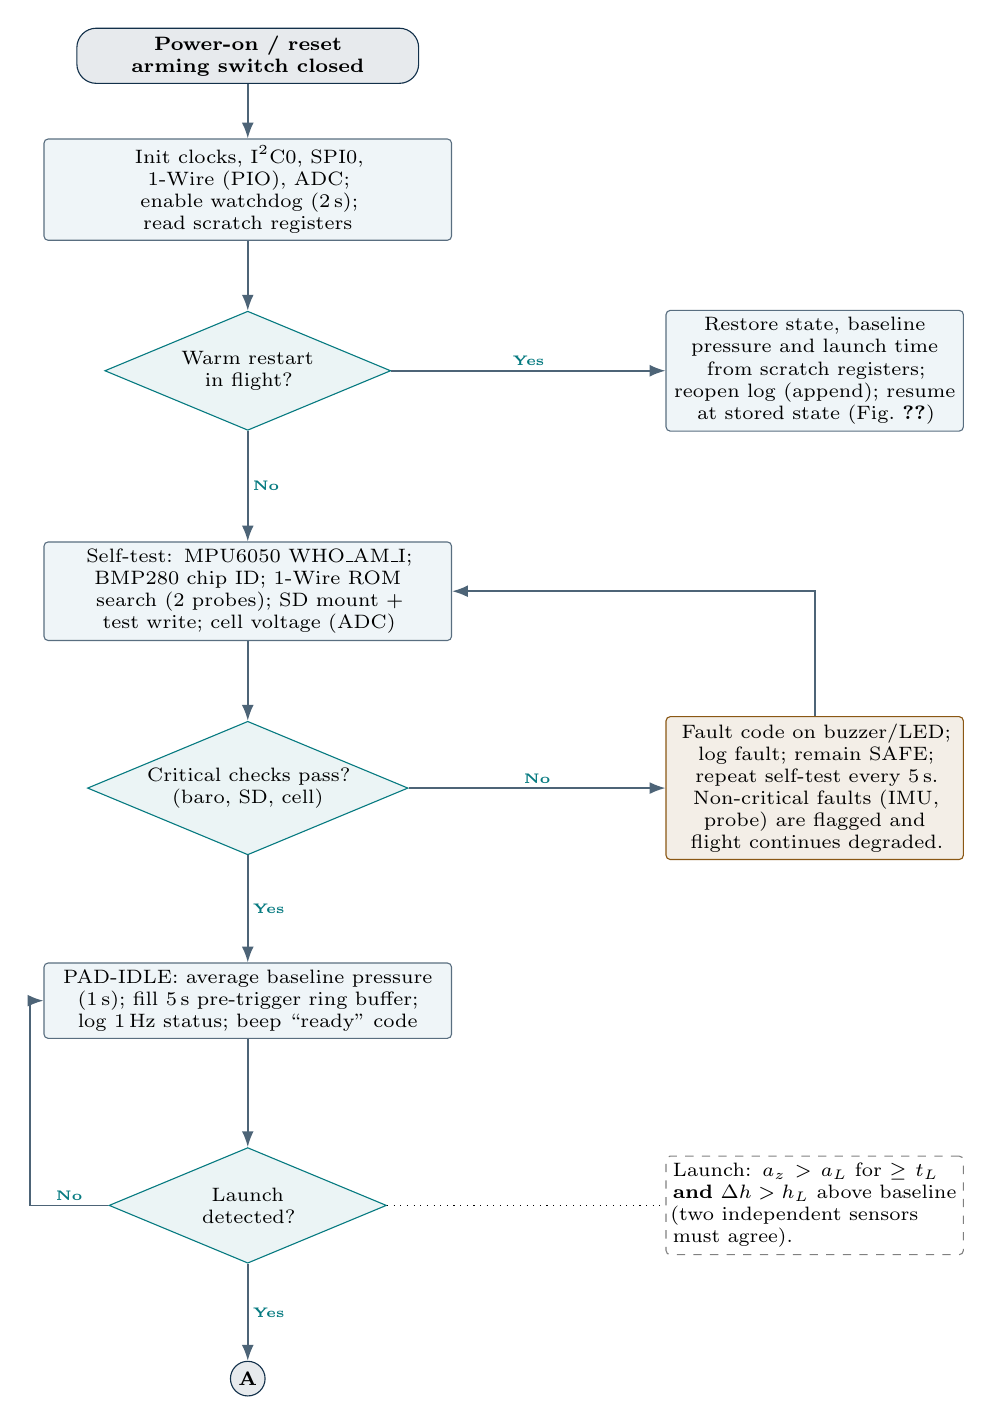
\begin{tikzpicture}
\node[term] (s) at (0,0) {Power-on / reset\\arming switch closed};
\node[proc] (boot) at (0,-1.7) {Init clocks, I$^2$C0, SPI0, 1-Wire (PIO), ADC;\\enable watchdog (2\,s); read scratch registers};
\node[dec] (d1) at (0,-4.0) {Warm restart\\in flight?};
\node[proc,text width=3.6cm] (rest) at (7.2,-4.0) {Restore state, baseline pressure and launch time from scratch registers; reopen log (append); resume at stored state (Fig.~\ref{fig:flight})};
\node[proc] (st) at (0,-6.8) {Self-test: MPU6050 WHO\_AM\_I; BMP280 chip ID; 1-Wire ROM search (2 probes); SD mount + test write; cell voltage (ADC)};
\node[dec,text width=2.6cm] (d2) at (0,-9.3) {Critical checks pass?\\(baro, SD, cell)};
\node[fault,text width=3.6cm] (f2) at (7.2,-9.3) {Fault code on buzzer/LED; log fault; remain SAFE; repeat self-test every 5\,s. Non-critical faults (IMU, probe) are flagged and flight continues degraded.};
\node[proc] (idle) at (0,-12.0) {PAD-IDLE: average baseline pressure (1\,s); fill 5\,s pre-trigger ring buffer; log 1\,Hz status; beep ``ready'' code};
\node[dec] (d3) at (0,-14.6) {Launch\\detected?};
\node[note,text width=3.6cm] (n3) at (7.2,-14.6) {Launch: $a_z>a_L$ for $\ge t_L$ \textbf{and} $\Delta h>h_L$ above baseline (two independent sensors must agree).};
\node[conn] (A) at (0,-16.8) {A};
\draw[flow] (s) -- (boot);
\draw[flow] (boot) -- (d1);
\draw[flow] (d1.east) -- node[lab,above]{Yes} (rest.west);
\draw[flow] (d1.south) -- node[lab,right]{No} (st.north);
\draw[flow] (st) -- (d2);
\draw[flow] (d2.east) -- node[lab,above]{No} (f2.west);
\draw[flow] (f2.north) |- (st.east);
\draw[flow] (d2.south) -- node[lab,right]{Yes} (idle.north);
\draw[flow] (idle) -- (d3);
\draw[flow] (d3.west) -- ++(-1.0,0) node[lab,above,pos=.5]{No} |- (idle.west);
\draw[dotted] (d3.east) -- (n3.west);
\draw[flow] (d3.south) -- node[lab,right]{Yes} (A.north);
\end{tikzpicture}
\caption{Logger Pico: start-up, warm-restart recovery, self-test and pad-idle until launch detect.}
\label{fig:boot}
\end{figure}

\begin{figure}[p]
\centering
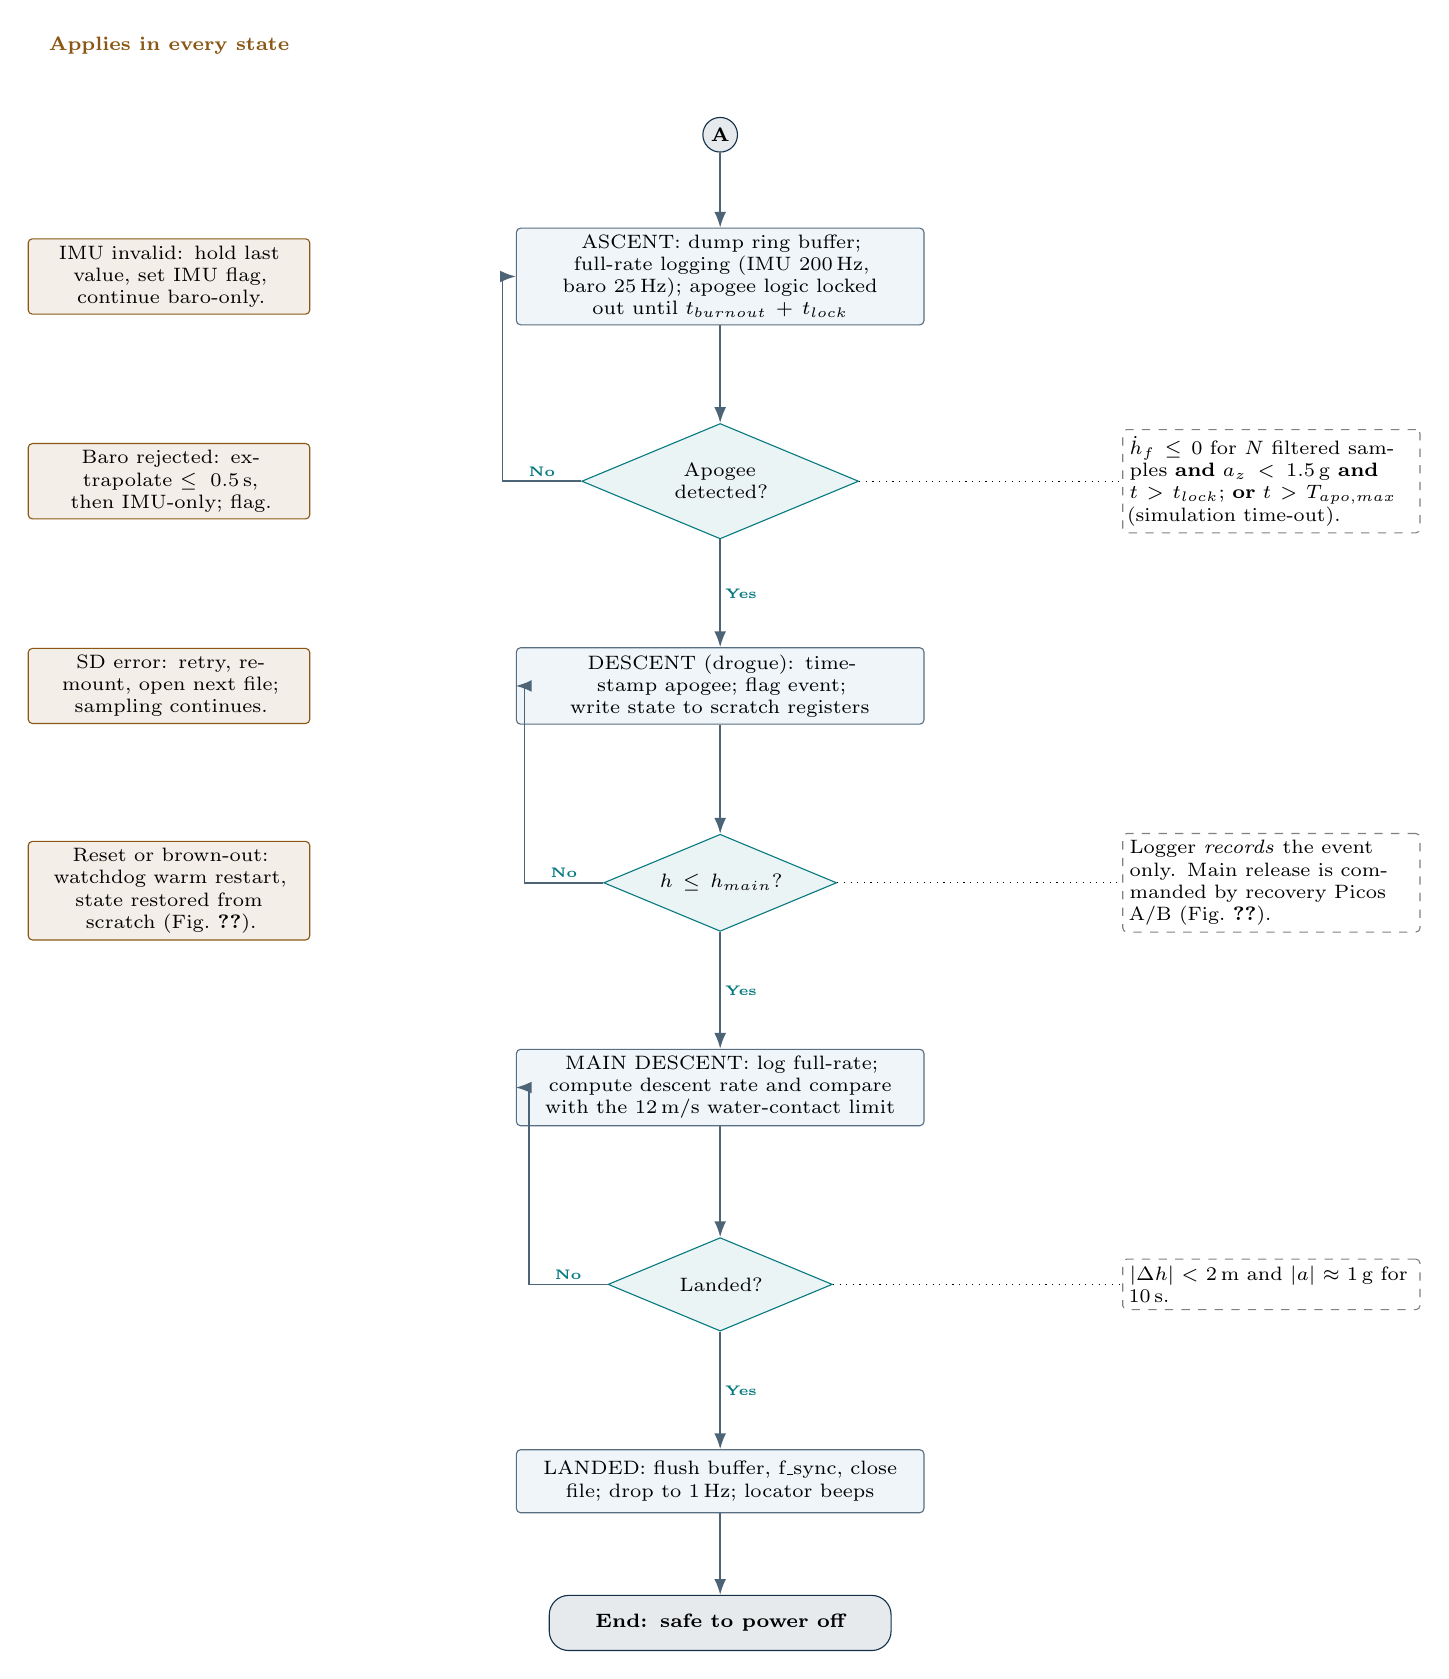
\begin{tikzpicture}
\node[font=\scriptsize\bfseries,color=Amber,anchor=south] at (-7.0,0.9) {Applies in every state};
\node[conn] (A) at (0,0) {A};
\node[proc] (asc) at (0,-1.8) {ASCENT: dump ring buffer; full-rate logging (IMU 200\,Hz, baro 25\,Hz); apogee logic locked out until $t_{burnout}+t_{lock}$};
\node[dec] (d4) at (0,-4.4) {Apogee\\detected?};
\node[note,text width=3.6cm] (n4) at (7.0,-4.4) {$\dot h_f\le0$ for $N$ filtered samples \textbf{and} $a_z<1.5$\,g \textbf{and} $t>t_{lock}$; \textbf{or} $t>T_{apo,max}$ (simulation time-out).};
\node[proc] (drog) at (0,-7.0) {DESCENT (drogue): time-stamp apogee; flag event; write state to scratch registers};
\node[dec] (d5) at (0,-9.5) {$h\le h_{main}$?};
\node[note,text width=3.6cm] (n5) at (7.0,-9.5) {Logger \emph{records} the event only. Main release is commanded by recovery Picos A/B (Fig.~\ref{fig:recovery}).};
\node[proc] (main) at (0,-12.1) {MAIN DESCENT: log full-rate; compute descent rate and compare with the 12\,m/s water-contact limit};
\node[dec] (d6) at (0,-14.6) {Landed?};
\node[note,text width=3.6cm] (n6) at (7.0,-14.6) {$|\Delta h|<2$\,m and $|a|\approx1$\,g for 10\,s.};
\node[proc] (land) at (0,-17.1) {LANDED: flush buffer, f\_sync, close file; drop to 1\,Hz; locator beeps};
\node[term] (end) at (0,-18.9) {End: safe to power off};
\node[fault] (a1) at (-7.0,-1.8) {IMU invalid: hold last value, set IMU flag, continue baro-only.};
\node[fault] (a2) at (-7.0,-4.4) {Baro rejected: extrapolate $\le0.5$\,s, then IMU-only; flag.};
\node[fault] (a3) at (-7.0,-7.0) {SD error: retry, remount, open next file; sampling continues.};
\node[fault] (a4) at (-7.0,-9.6) {Reset or brown-out: watchdog warm restart, state restored from scratch (Fig.~\ref{fig:boot}).};
\draw[flow] (A) -- (asc);
\draw[flow] (asc) -- (d4);
\draw[flow] (d4.south) -- node[lab,right]{Yes} (drog.north);
\draw[flow] (d4.west) -- ++(-1.0,0) node[lab,above,pos=.5]{No} |- (asc.west);
\draw[dotted] (d4.east) -- (n4.west);
\draw[flow] (drog) -- (d5);
\draw[flow] (d5.south) -- node[lab,right]{Yes} (main.north);
\draw[flow] (d5.west) -- ++(-1.0,0) node[lab,above,pos=.5]{No} |- (drog.west);
\draw[dotted] (d5.east) -- (n5.west);
\draw[flow] (main) -- (d6);
\draw[flow] (d6.south) -- node[lab,right]{Yes} (land.north);
\draw[flow] (d6.west) -- ++(-1.0,0) node[lab,above,pos=.5]{No} |- (main.west);
\draw[dotted] (d6.east) -- (n6.west);
\draw[flow] (land) -- (end);
\end{tikzpicture}
\caption{Logger Pico in-flight state machine. Left column: anomaly handling that applies in all states.}
\label{fig:flight}
\end{figure}

\begin{figure}[p]
\centering
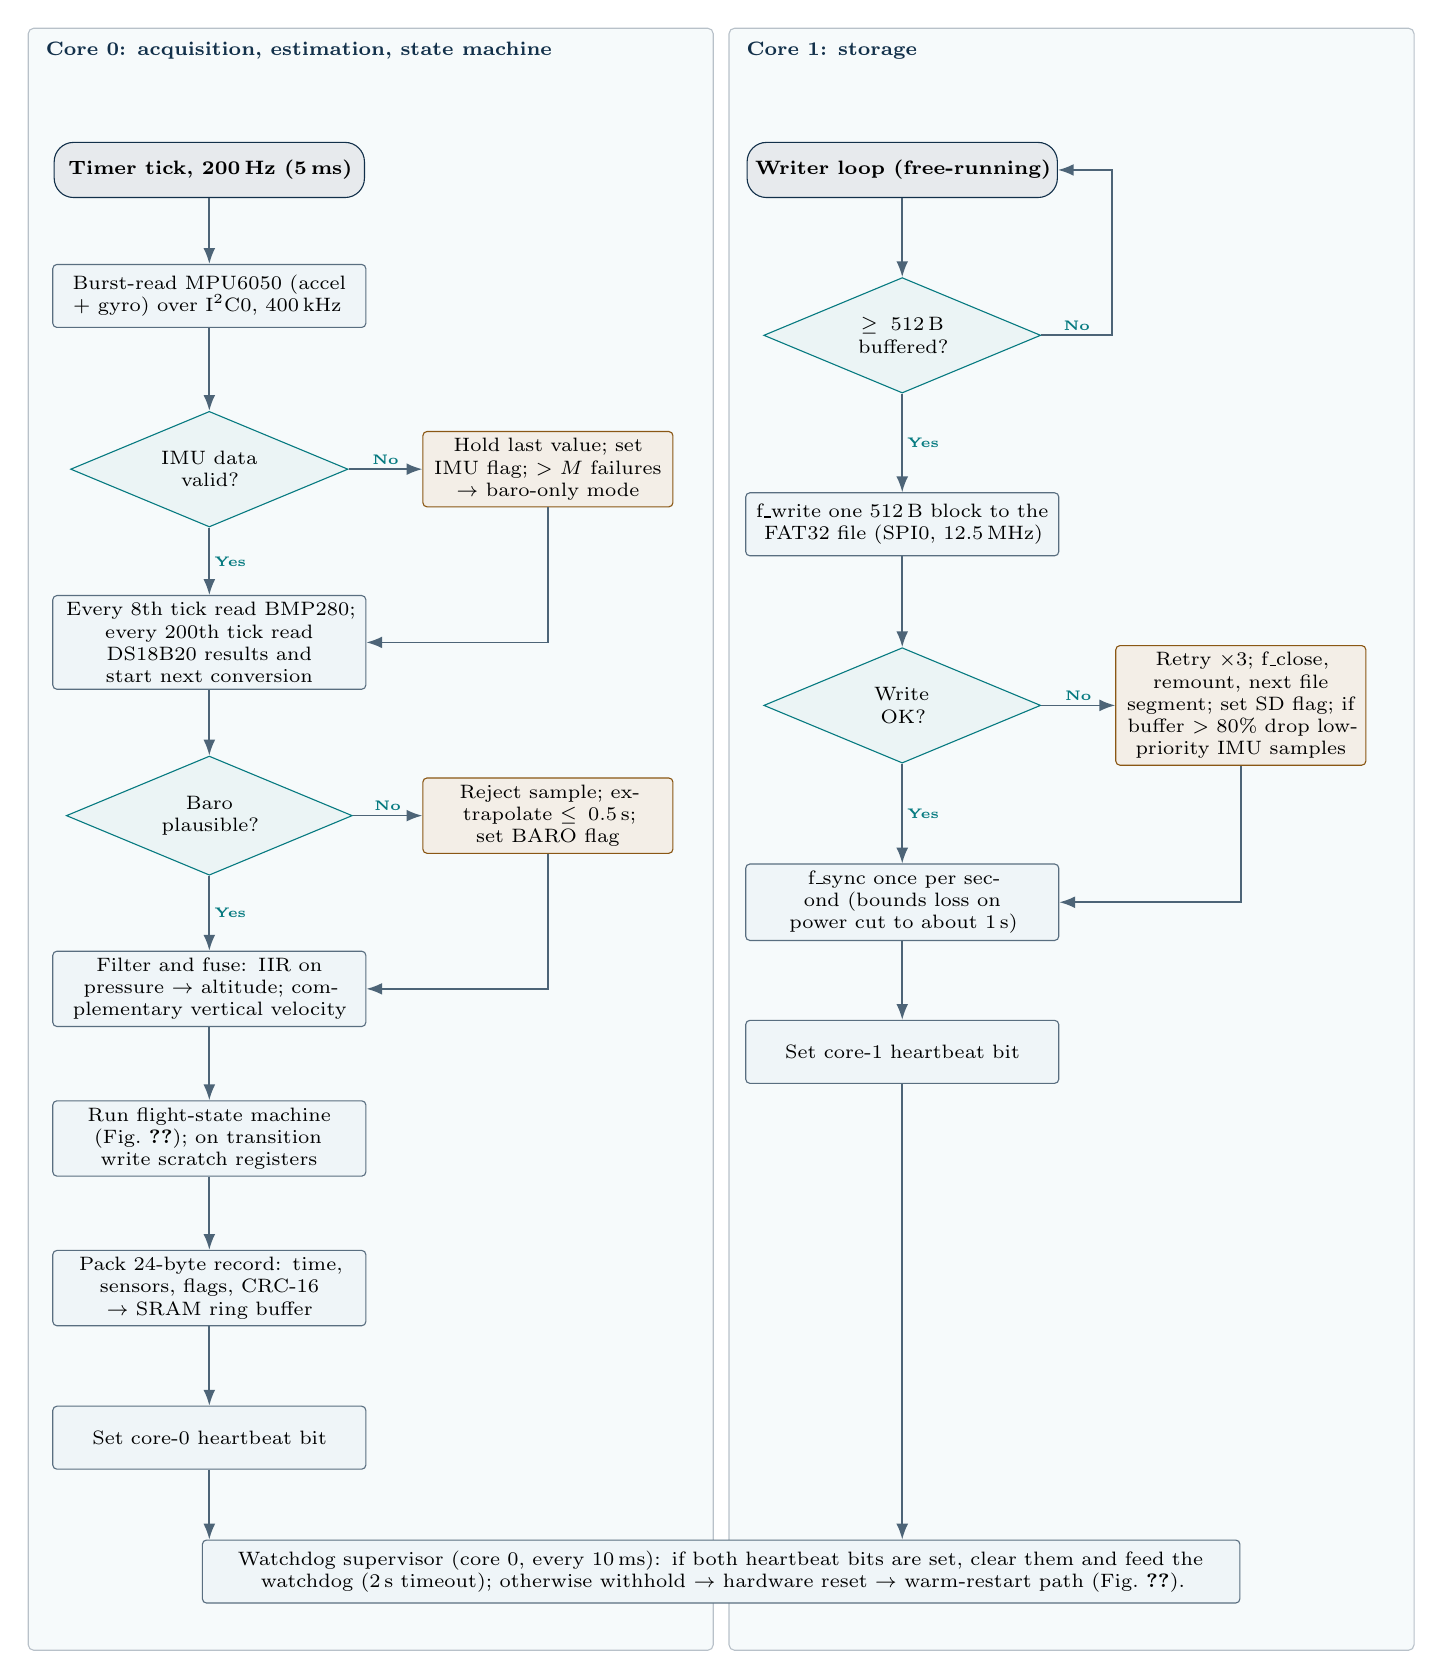
\begin{tikzpicture}
\draw[lane] (-8.8,0.9) rectangle (-0.1,-19.7);
\draw[lane] (0.1,0.9) rectangle (8.8,-19.7);
\node[font=\scriptsize\bfseries,color=Navy,anchor=north west] at (-8.7,0.85) {Core 0: acquisition, estimation, state machine};
\node[font=\scriptsize\bfseries,color=Navy,anchor=north west] at (0.2,0.85) {Core 1: storage};
% core 0
\node[term,text width=3.8cm] (t0) at (-6.5,-0.9) {Timer tick, 200\,Hz (5\,ms)};
\node[proc,text width=3.8cm] (imu) at (-6.5,-2.5) {Burst-read MPU6050 (accel + gyro) over I$^2$C0, 400\,kHz};
\node[dec] (di) at (-6.5,-4.7) {IMU data\\valid?};
\node[fault,text width=3.0cm] (fi) at (-2.2,-4.7) {Hold last value; set IMU flag; $>M$ failures $\rightarrow$ baro-only mode};
\node[proc,text width=3.8cm] (bar) at (-6.5,-6.9) {Every 8th tick read BMP280; every 200th tick read DS18B20 results and start next conversion};
\node[dec] (db) at (-6.5,-9.1) {Baro\\plausible?};
\node[fault,text width=3.0cm] (fb) at (-2.2,-9.1) {Reject sample; extrapolate $\le0.5$\,s; set BARO flag};
\node[proc,text width=3.8cm] (fil) at (-6.5,-11.3) {Filter and fuse: IIR on pressure $\rightarrow$ altitude; complementary vertical velocity};
\node[proc,text width=3.8cm] (fsm) at (-6.5,-13.2) {Run flight-state machine (Fig.~\ref{fig:flight}); on transition write scratch registers};
\node[proc,text width=3.8cm] (pk) at (-6.5,-15.1) {Pack 24-byte record: time, sensors, flags, CRC-16 $\rightarrow$ SRAM ring buffer};
\node[proc,text width=3.8cm] (hb0) at (-6.5,-17.0) {Set core-0 heartbeat bit};
% core 1
\node[term,text width=3.8cm] (w0) at (2.3,-0.9) {Writer loop (free-running)};
\node[dec] (wd) at (2.3,-3.0) {$\ge512$\,B\\buffered?};
\node[proc,text width=3.8cm] (wr) at (2.3,-5.4) {f\_write one 512\,B block to the FAT32 file (SPI0, 12.5\,MHz)};
\node[dec] (dw) at (2.3,-7.7) {Write\\OK?};
\node[fault,text width=3.0cm] (fw) at (6.6,-7.7) {Retry $\times3$; f\_close, remount, next file segment; set SD flag; if buffer $>80\%$ drop low-priority IMU samples};
\node[proc,text width=3.8cm] (sy) at (2.3,-10.2) {f\_sync once per second (bounds loss on power cut to about 1\,s)};
\node[proc,text width=3.8cm] (hb1) at (2.3,-12.1) {Set core-1 heartbeat bit};
% supervisor
\node[proc,text width=13cm] (sup) at (0,-18.7) {Watchdog supervisor (core 0, every 10\,ms): if both heartbeat bits are set, clear them and feed the watchdog (2\,s timeout); otherwise withhold $\rightarrow$ hardware reset $\rightarrow$ warm-restart path (Fig.~\ref{fig:boot}).};
% flows core 0
\draw[flow] (t0) -- (imu);
\draw[flow] (imu) -- (di);
\draw[flow] (di.south) -- node[lab,right]{Yes} (bar.north);
\draw[flow] (di.east) -- node[lab,above]{No} (fi.west);
\draw[flow] (fi.south) |- (bar.east);
\draw[flow] (bar) -- (db);
\draw[flow] (db.south) -- node[lab,right]{Yes} (fil.north);
\draw[flow] (db.east) -- node[lab,above]{No} (fb.west);
\draw[flow] (fb.south) |- (fil.east);
\draw[flow] (fil) -- (fsm);
\draw[flow] (fsm) -- (pk);
\draw[flow] (pk) -- (hb0);
\draw[flow] (hb0.south) -- (hb0.south |- sup.north);
% flows core 1
\draw[flow] (w0) -- (wd);
\draw[flow] (wd.east) -- ++(0.9,0) node[lab,above,pos=.5]{No} |- (w0.east);
\draw[flow] (wd.south) -- node[lab,right]{Yes} (wr.north);
\draw[flow] (wr) -- (dw);
\draw[flow] (dw.south) -- node[lab,right]{Yes} (sy.north);
\draw[flow] (dw.east) -- node[lab,above]{No} (fw.west);
\draw[flow] (fw.south) |- (sy.east);
\draw[flow] (sy) -- (hb1);
\draw[flow] (hb1.south) -- (hb1.south |- sup.north);
\end{tikzpicture}
\caption{Logger Pico dual-core task flow with fault handling and the cross-core watchdog supervisor. Core~1 absorbs SD latency so core~0 timing is never blocked.}
\label{fig:loop}
\end{figure}

\begin{figure}[p]
\centering
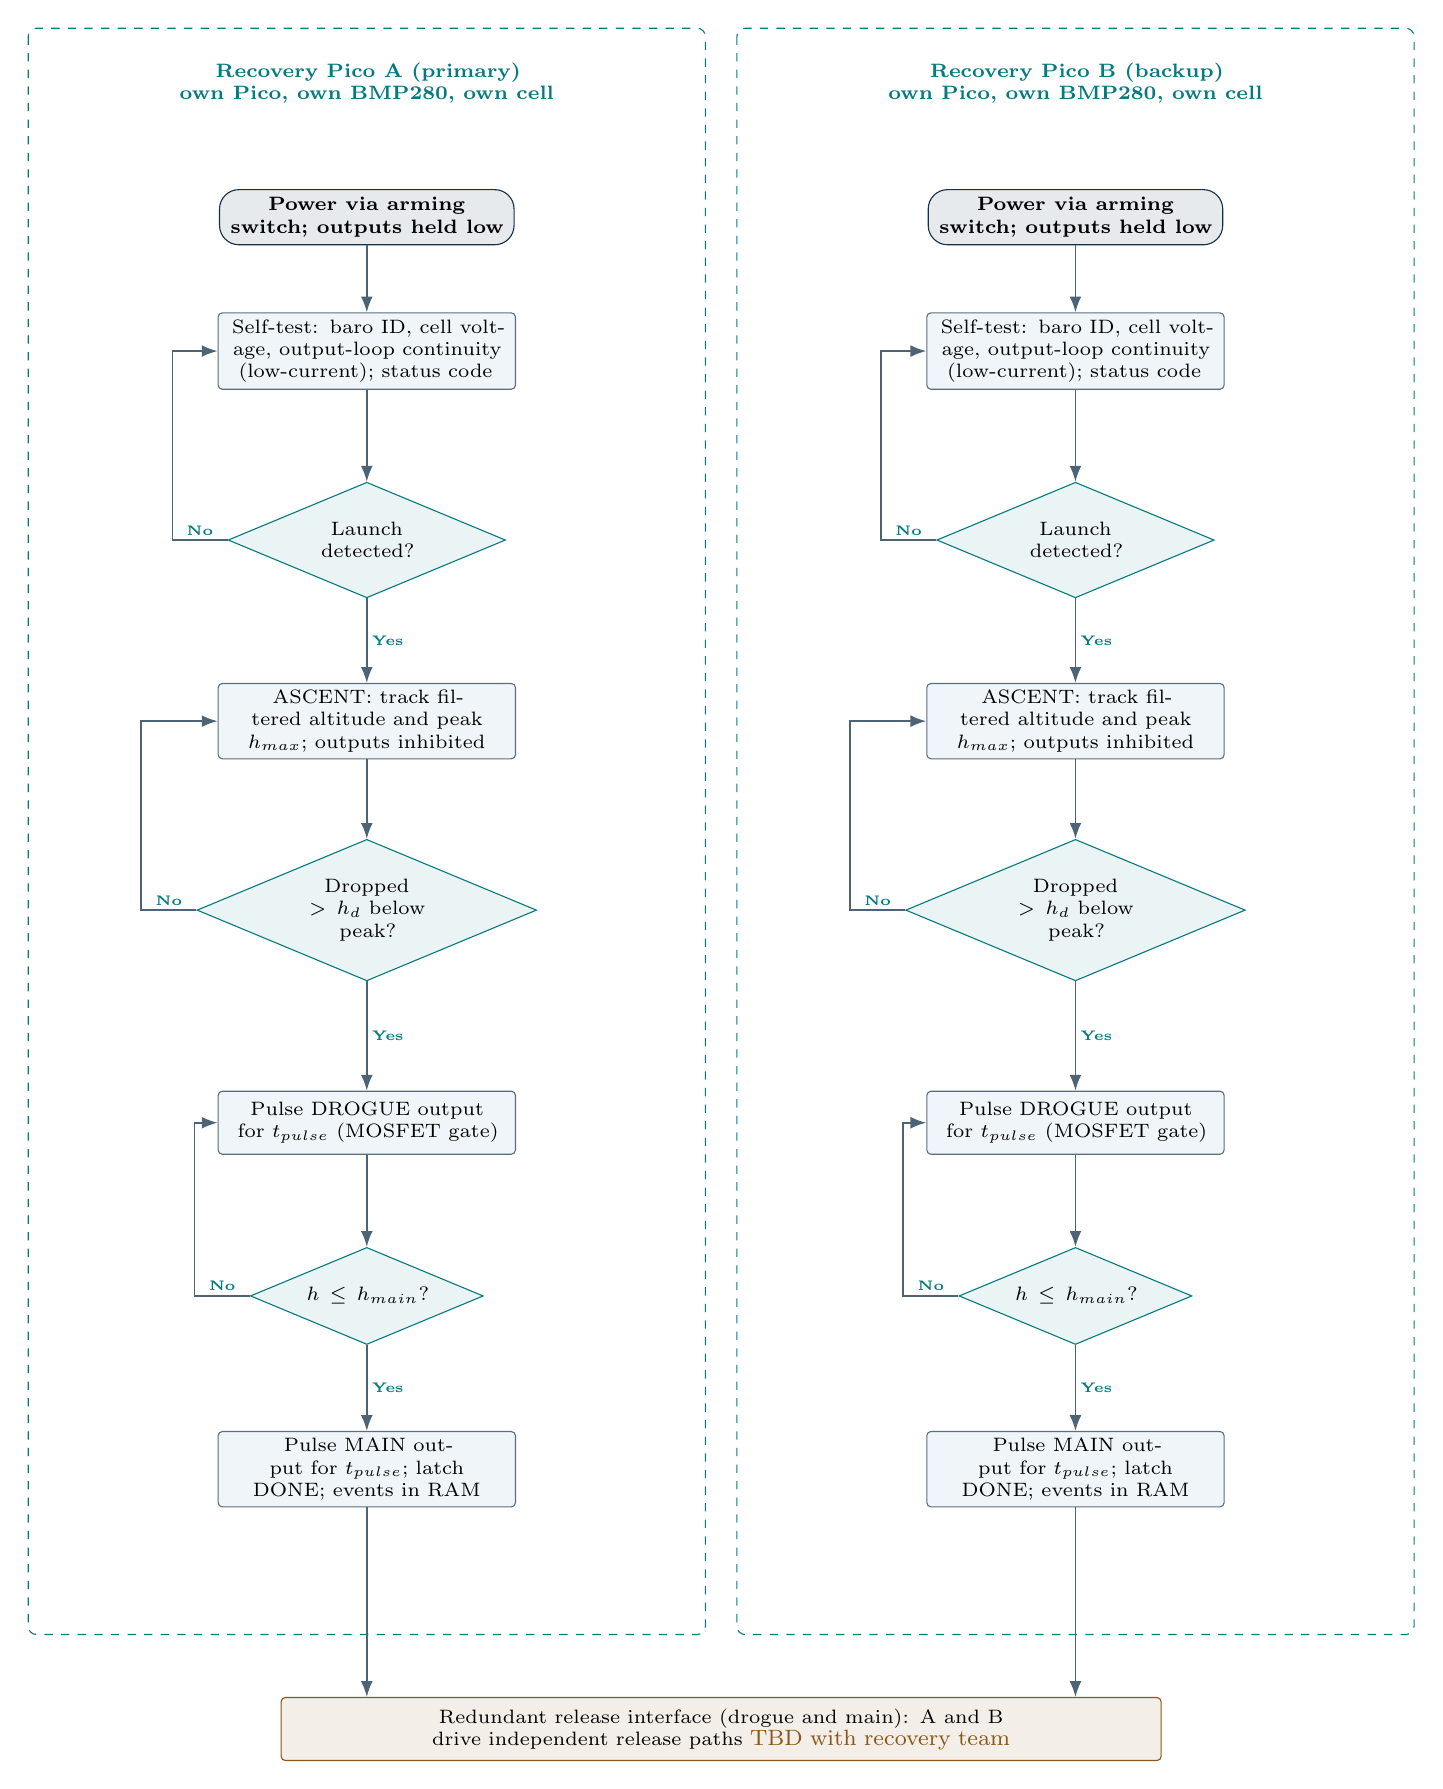
\begin{tikzpicture}
\draw[group] (-8.8,1.9) rectangle (-0.2,-18.5);
\draw[group] (0.2,1.9) rectangle (8.8,-18.5);
\node[font=\scriptsize\bfseries,color=Teal,align=center,text width=8cm] at (-4.5,1.2) {Recovery Pico A (primary)\\own Pico, own BMP280, own cell};
\node[font=\scriptsize\bfseries,color=Teal,align=center,text width=8cm] at (4.5,1.2) {Recovery Pico B (backup)\\own Pico, own BMP280, own cell};
\foreach \n/\x in {A/-4.5, B/4.5} {
  \node[term,text width=3.6cm] (s0\n) at (\x,-0.5) {Power via arming switch; outputs held low};
  \node[proc,text width=3.6cm] (s1\n) at (\x,-2.2) {Self-test: baro ID, cell voltage, output-loop continuity (low-current); status code};
  \node[dec] (d1\n) at (\x,-4.6) {Launch\\detected?};
  \node[proc,text width=3.6cm] (s2\n) at (\x,-6.9) {ASCENT: track filtered altitude and peak $h_{max}$; outputs inhibited};
  \node[dec] (d2\n) at (\x,-9.3) {Dropped\\$>h_d$ below\\peak?};
  \node[proc,text width=3.6cm] (s3\n) at (\x,-12.0) {Pulse DROGUE output for $t_{pulse}$ (MOSFET gate)};
  \node[dec] (d3\n) at (\x,-14.2) {$h\le h_{main}$?};
  \node[proc,text width=3.6cm] (s4\n) at (\x,-16.4) {Pulse MAIN output for $t_{pulse}$; latch DONE; events in RAM};
  \draw[flow] (s0\n) -- (s1\n);
  \draw[flow] (s1\n) -- (d1\n);
  \draw[flow] (d1\n.south) -- node[lab,right]{Yes} (s2\n.north);
  \draw[flow] (d1\n.west) -- ++(-0.7,0) node[lab,above,pos=.5]{No} |- (s1\n.west);
  \draw[flow] (s2\n) -- (d2\n);
  \draw[flow] (d2\n.south) -- node[lab,right]{Yes} (s3\n.north);
  \draw[flow] (d2\n.west) -- ++(-0.7,0) node[lab,above,pos=.5]{No} |- (s2\n.west);
  \draw[flow] (s3\n) -- (d3\n);
  \draw[flow] (d3\n.south) -- node[lab,right]{Yes} (s4\n.north);
  \draw[flow] (d3\n.west) -- ++(-0.7,0) node[lab,above,pos=.5]{No} |- (s3\n.west);
}
\node[fault,text width=11cm] (act) at (0,-19.7) {Redundant release interface (drogue and main): A and B drive independent release paths \status{TBD with recovery team}};
\draw[flow] (s4A.south) -- (s4A.south |- act.north);
\draw[flow] (s4B.south) -- (s4B.south |- act.north);
\end{tikzpicture}
\caption{Independent recovery controllers. B uses a later apogee trigger and a lower main altitude than A (Sec.~\ref{tab:params}), so a single common-mode threshold error does not trip both at the same instant.}
\label{fig:recovery}
\end{figure}

\subsection{Decision parameters (initial placeholders pending simulation)}
\small
\rowcolors{2}{Pale}{white}
\begin{longtable}{@{}L{22mm}L{58mm}L{66mm}@{}}
\toprule\rowcolor{VeryLight}\textbf{Symbol}&\textbf{Meaning}&\textbf{Starting value / source}\\\midrule\endfirsthead
\toprule\rowcolor{VeryLight}\textbf{Symbol}&\textbf{Meaning}&\textbf{Starting value}\\\midrule\endhead
\bottomrule\endlastfoot
$a_L$, $t_L$ & Launch acceleration threshold and duration (logger and recovery). & e.g.\ 2.5\,g for 50\,ms (10 IMU samples); set from motor thrust-to-weight in simulation.\\
$h_L$ & Altitude rise confirming launch. & e.g.\ 10\,m above baseline within 2\,s.\\
$t_{lock}$ & Apogee lock-out after burnout. & Simulation-derived, e.g.\ 1--2\,s, to avoid pressure disturbances near burnout/transonic flight.\\
$N$ & Consecutive filtered samples with $\dot h_f\le0$. & 5 samples at 25\,Hz (0.2\,s).\\
$T_{apo,max}$ & Apogee time-out from launch. & Simulated apogee time $+$ margin.\\
$h_d$ (A / B) & Drop below peak that confirms apogee on recovery boards. & A: small (e.g.\ 3\,m); B: larger (e.g.\ 8\,m) plus delay $\Delta t_B$.\\
$h_{main}$ (A / B) & Main-parachute deployment altitude (AGL). & Within 150--450\,m \cite{rtc2027app03,rtc2027app08}; B set about 30\,m lower than A.\\
$t_{pulse}$ & Output pulse duration. & From release-device specification \status{TBD}.\\
$v_{max}$ & Baro plausibility limit on $|dh/dt|$. & Simulated peak speed $\times$ margin \status{TBD}.\\
\end{longtable}
\normalsize
\label{tab:params}

%======================================================================
\section{Robustness and fault handling}
%======================================================================
\small
\rowcolors{2}{Pale}{white}
\begin{longtable}{@{}L{34mm}L{50mm}L{62mm}@{}}
\toprule\rowcolor{VeryLight}\textbf{Failure mode}&\textbf{Consequence}&\textbf{Mitigation (see flowcharts)}\\\midrule\endfirsthead
\toprule\rowcolor{VeryLight}\textbf{Failure mode}&\textbf{Consequence}&\textbf{Mitigation}\\\midrule\endhead
\bottomrule\endlastfoot
Logger power dip or lockup & Gaps in data or payload record. & Watchdog + scratch-register warm restart; 1\,s sync; protected supply.\\
Barometer noise, spike or port blockage & False apogee or main trigger. & Plausibility gate, IIR filter, multi-condition apogee, lock-out, time-out.\\
IMU saturation & Bad launch/burnout and acceleration data. & Baro cross-check, $\pm200$\,g option \cite{adxl375ds}, flags in record.\\
SD write stall or removal & Missing records. & Core-1 offload, 24\,kB buffer, retry/remount, next-file segment.\\
Recovery A failure & No or late deployment. & Backup B: separate board, sensor, cell, later trigger.\\
Premature output from noise/boot & Unsafe activation. & Outputs held low by pull-downs, arming switch, launch-inhibit logic.\\
Thermal probe detaches & Invalid payload data; loose object. & Mechanical retention, strain relief, flag in record.\\
Connector loosening & Intermittent power/data. & Locking connectors, strain relief, vibration test \cite{rtc2027app03}.\\
\end{longtable}
\normalsize
The full FMEA follows the organiser template \cite{rtc2027app12}; classical FMECA practice is described in \cite{mil1629a}.

%======================================================================
\section{Power and data budgets}
\label{sec:power}
%======================================================================
\textbf{Load estimate (logger).} Values are datasheet-typical or assumed, and must be replaced by measurements.

\small
\rowcolors{2}{Pale}{white}
\begin{tabularx}{\linewidth}{@{}L{48mm}r Y@{}}
\toprule\rowcolor{VeryLight}\textbf{Item}&\textbf{mA}&\textbf{Basis}\\\midrule
Pico L at 125\,MHz, both cores & 30 & Assumed; measure \cite{rp2040ds}\\
MPU6050 (gyro + accel) & 3.9 & Datasheet typical \cite{mpu6050ds}\\
BMP280 & $<0.1$ & Datasheet \cite{bmp280ds}\\
2$\times$ DS18B20 active & 2 & About 1\,mA each \cite{ds18b20ds}\\
microSD module average & 20 & Assumed; write peaks higher\\
\midrule
\textbf{Total estimate} & \textbf{$\approx$56} & Design basis kept at \textbf{200\,mA}\\
\bottomrule
\end{tabularx}
\normalsize

At 56\,mA the 1.5\,h minimum \cite{rtc2027app03} needs about 84\,mAh. Using the conservative 200\,mA at 3.3\,V through an assumed 85\% efficient converter, the demand is $3.3\times0.2\times1.5/0.85\approx1.16$\,Wh, against about 9.6\,Wh stored in a nominal 3.7\,V, 2.6\,Ah cell ($\approx$8$\times$ margin). The margin is only a sizing indicator; a measured endurance test of more than 1.5\,h is required. Recovery boards use the same method plus the release-device pulse load \status{TBD}.

\textbf{Data budget.} 24\,B $\times$ 200\,Hz = 4.8\,kB/s; 90\,min $=5400$\,s $\Rightarrow$ about 26\,MB. SPI at 12.5\,MHz and 512\,B block writes leave large margin, and the 24\,kB buffer covers about 5\,s of SD latency.

%======================================================================
\section{Verification plan}
%======================================================================
Methods follow the usual inspection, analysis, demonstration and test categories \cite{nasase}; MDR needs the plan, not the results \cite{rtc2027app07}.

\small
\rowcolors{2}{Pale}{white}
\begin{tabularx}{\linewidth}{@{}L{12mm}L{24mm}Y@{}}
\toprule\rowcolor{VeryLight}\textbf{ID}&\textbf{Method}&\textbf{Planned evidence}\\\midrule
V-01 & Test & Replay recorded and simulated altitude/acceleration histories through the state machine; check false-apogee and main-trigger margins.\\
V-02 & Test & Logger timing: loop jitter, buffer occupancy and SD latency under load; forced SD errors.\\
V-03 & Demonstration & Watchdog test: force a core stall mid-sequence and confirm state restore and log continuity.\\
V-04 & Demonstration & Recovery A and B each switch safe test loads independently; confirm outputs stay low through power-up, reset and brown-out.\\
V-05 & Test & Power endurance $>1.5$\,h with realistic logging; connector pull and vibration retention.\\
V-06 & Test & Thermal probes at reference temperature points; data completeness and time alignment.\\
V-07 & Test & Barometer port: pressure-chamber or vented-bay test with representative pressure profile.\\
V-08 & Inspection & Wiring, labels, strain relief, arming-switch access and polarity \cite{rtc2027app03}.\\
V-09 & Analysis & Mass, power and cost budget and FMEA update for PDR \cite{rtc2027app12}.\\
\bottomrule
\end{tabularx}
\normalsize

%======================================================================
\section{Decisions needed from the team}
%======================================================================
\begin{enumerate}
\item Approve a three-Pico architecture (logger + two recovery), or choose an alternative recovery controller while keeping the same independence rules.
\item Obtain simulated peak acceleration, speed, apogee time and apogee altitude to fix $a_L$, $t_{lock}$, $v_{max}$, $T_{apo,max}$ and the IMU range.
\item Define the release mechanism with the recovery lead and organiser requirements; replace \status{TBD} items with specifications and quotes.
\item Confirm bay dimensions, mounting, battery protection and measured current before procurement.
\item Confirm the official GPS beacon ownership and cost.
\end{enumerate}

\printbibliography[title={References}]
\end{document}